% !TeX root = ../main.tex
\section{Introduction}
\label{sec:intro}
With the growth of e-commerce and digital services, recommender systems have become essential infrastructure for online platforms. However, traditional recommender systems typically consolidate vast amounts of user data centrally, leading to privacy and regulatory concerns. Federated learning allows multiple clients to collaboratively train a model without sharing raw data; federated recommendation (FR) applies this idea to recommendation, where interaction histories remain on local devices and only model parameters are aggregated~\citep{ammad2019federated,mcmahan2017communication}.

Meanwhile, cross-domain transfer is another longstanding need: platforms wish to reuse a mature catalog to bootstrap a new service, where newly listed items lack behavioral evidence. However, existing cross-domain recommenders typically assume overlapping users or alignable item identifiers, and neither premise holds under federated constraints---participating services cannot pool user histories, and disjoint catalogs share no identifiers to align. We study this disjoint-catalog setting without requiring linked users between source and target domains.

A viable route is offered by pretrained text encoders: items from different catalogs are mapped into a common semantic space, enabling transfer without matching identifiers~\citep{zhang2026transfr}. However, the semantic space alone does not resolve the uneven supervision of the target domain. On the one hand, frequently observed items supply many ranking constraints, whereas rare items provide little evidence for adaptation; on the other hand, clients observe different semantic regions through their own histories, so a globally rare item may be familiar to one client yet unseen by another. Moreover, excessive adaptation drifts representations away from the pretrained semantics, harming items with scarce evidence. An adaptation rule therefore needs to account for the amount of item-level evidence, the client context in which it is observed, and how much of the pretrained prior should be preserved.

Personalized adapters and expert mixtures address variation across clients~\citep{li2026fedvlr,li2026fedpa}, but client-level personalization does not by itself specify how items with different training frequencies should share adaptation paths: a single shared transformation applies the same parameterization to all items, and an additional adapter introduces capacity without determining how to allocate it. In this light, we use item frequency as an observable proxy for the available target supervision, route each item between two residual paths, and adjust the routed representation to the local interaction profile through client conditioning.

To address the challenges mentioned above, we propose FedPASA, which combines three operations in a shared semantic adapter. Specifically, Popularity-Gated Dual-path Routing (PGDR) mixes a source-initialized path and a target-initialized path using a frequency-derived weight; client conditioning produces feature-wise scales and shifts from a locally pooled semantic profile; in addition, AutoAnchor interpolates the resulting representation with the frozen text embedding, with the anchor strength set by a catalog-level user-to-item ratio. Both residual paths are updated on the target domain, while source initialization provides a starting point rather than a fixed representation.

We evaluate this design on multiple real-world datasets, with controls that separate frequency assignment, model capacity, and final personalization. Our contributions are summarized as follows:
\begin{itemize}
\item We propose FedPASA, a reliability-aware semantic adaptation framework that adjusts item representations according to evidence strength at the item, client, and catalog levels. Our framework is motivated by an analysis of the failure of uniform adaptation in existing federated semantic transfer methods under uneven target supervision: a single shared transformation underfits well-supported frequent items while overfitting sparsely observed items. The proposed framework applies to different backbone encoders.
\item We design PGDR to combine two trainable residual adaptation paths using frequency-derived weights, without an additional learned routing network. Client conditioning adjusts the combined representations using local semantic profiles, while AutoAnchor controls their mixture with the frozen semantic prior through a catalog-level rule.
\item We conduct extensive experiments on multiple real-world datasets. With the same text encoder, FedPASA achieves higher average cross-domain recommendation accuracy than the evaluated baselines. Comparisons that retain the same network structure and parameter count further show that frequency-derived mixing weights outperform using a common pair of weights for all items or shuffling the item--weight assignments. Ablation studies further characterize the effects of individual components.
\end{itemize}

\par\addvspace{6pt}\noindent\begin{minipage}{\columnwidth}
\centering
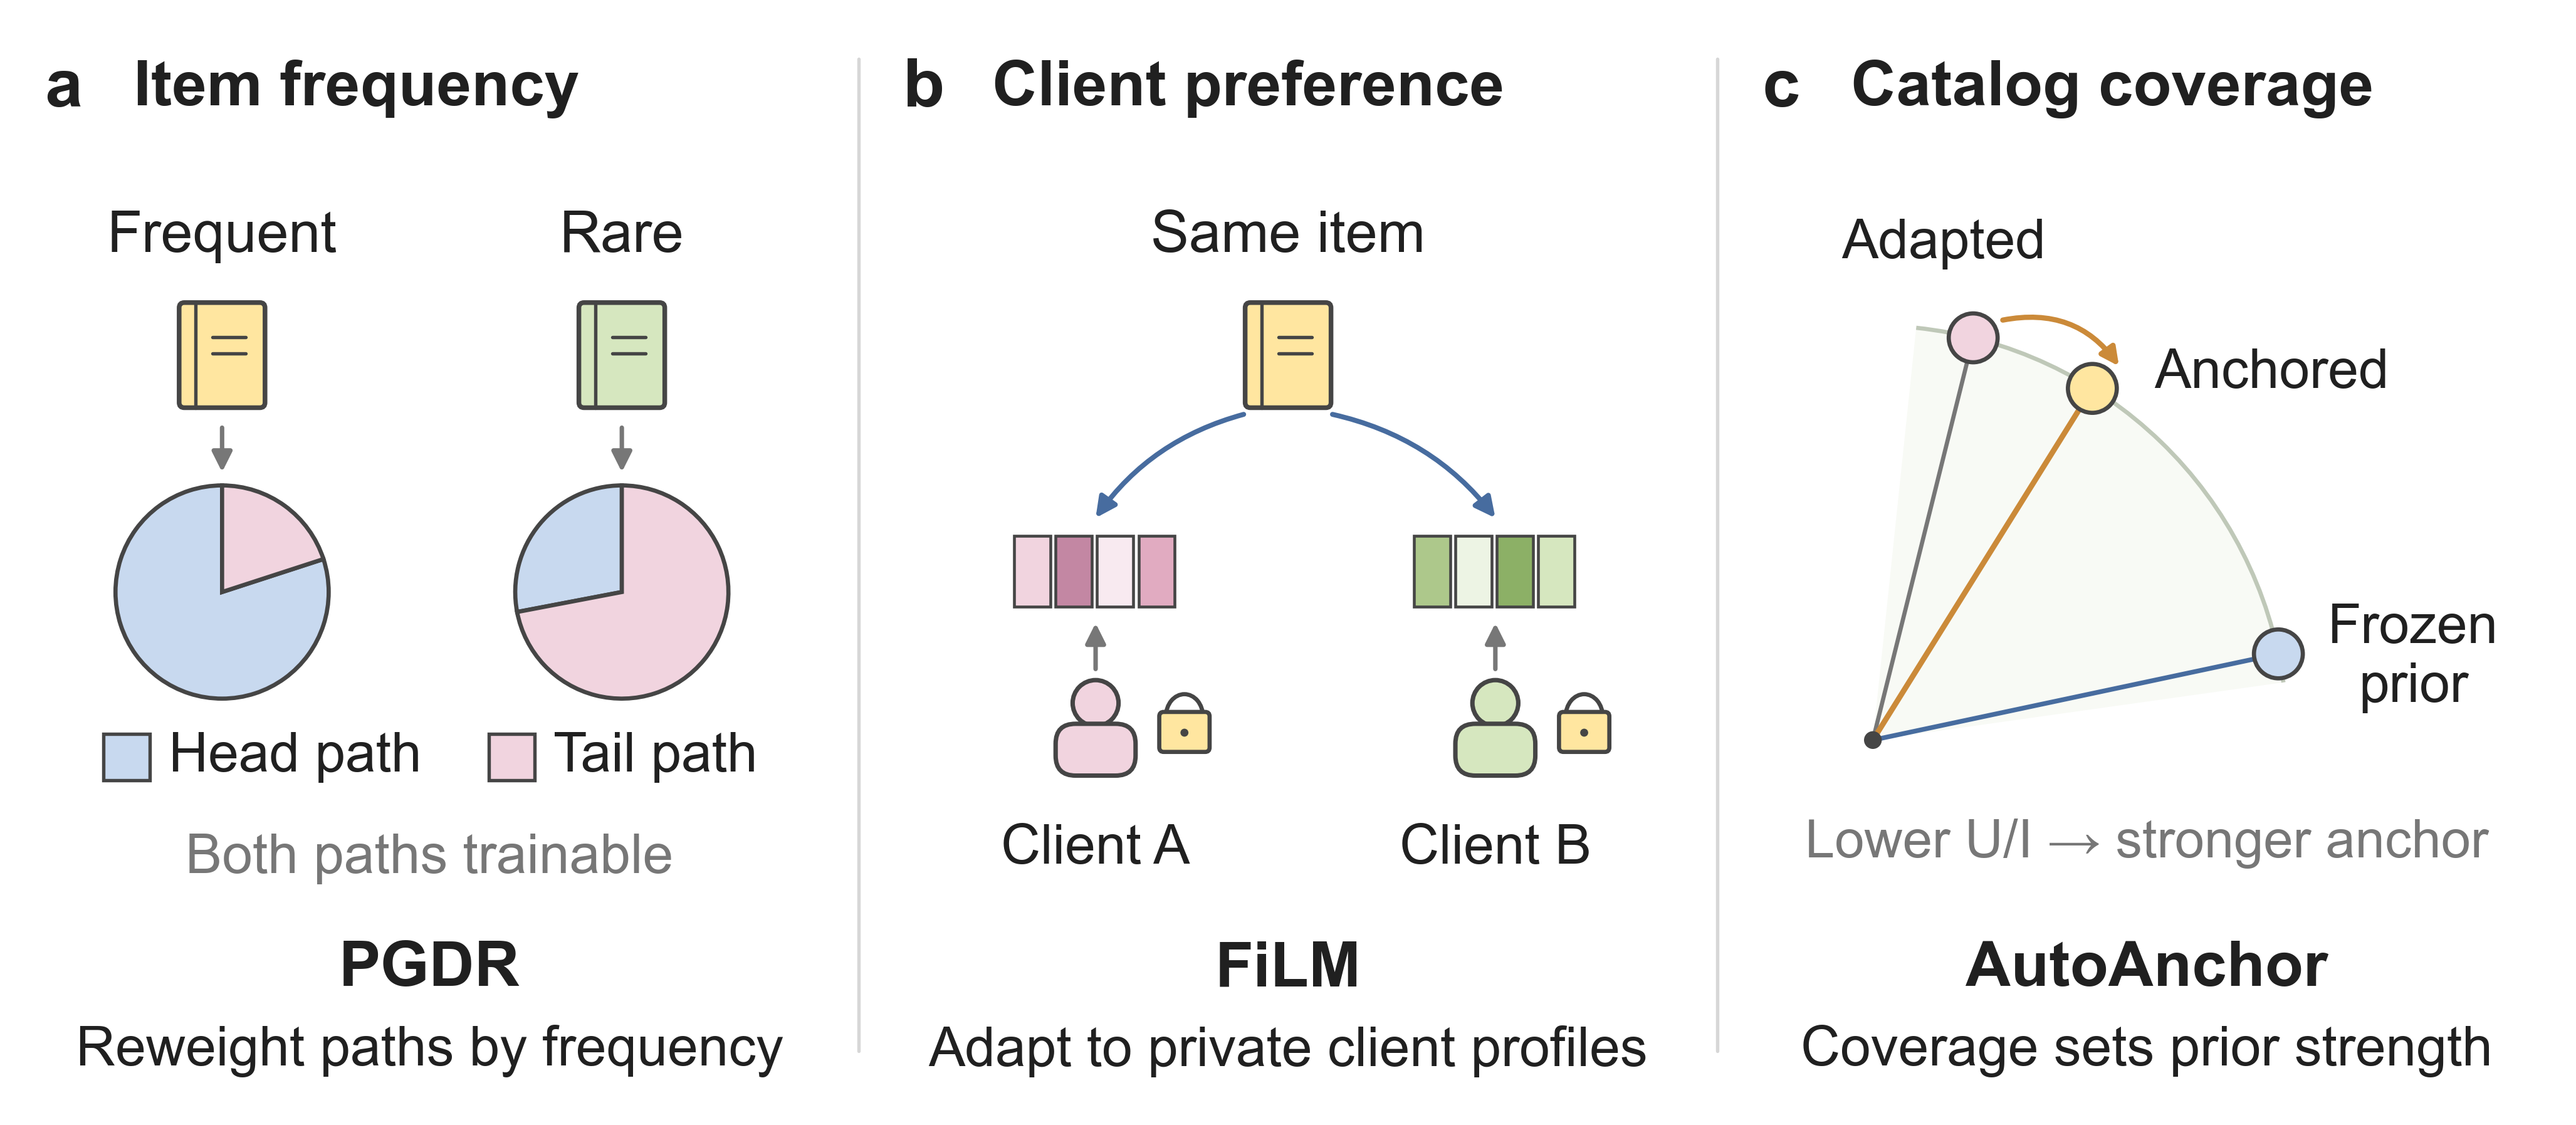
\includegraphics[width=\linewidth]{figures/adaptation_overview.png}
\captionof{figure}{Three adaptation controls: (a) frequency-based path mixing; (b) private-profile conditioning; (c) catalog-dependent prior preservation.}
\label{fig:adaptation-overview}
\end{minipage}\par\addvspace{6pt}

